\documentclass{article}

\usepackage{svg}
\usepackage{microtype}
\usepackage[framemethod=tikz]{mdframed}
\usepackage{hyperref}
\usepackage{url}
\usepackage{xspace}
\hypersetup{
    colorlinks,
    citecolor=black,
    filecolor=black,
    linkcolor=black,
    urlcolor=black
}

\author{Zanella Mioso}

\title{Documentazione progetto Ingegneria del Software}

\begin{document}

\maketitle

\newpage

\tableofcontents

\newpage

\section{Requisiti ed interazioni utente-sistema}

\subsection{Specifiche casi d’uso}

Il sistema è diviso in due parti principali. Una dedicata all'utente e l'altra
al responsabile del reparto. Per \textbf{utente} si intende la persona che utlilizza questo
servizio per fare la spesa e per \textbf{responsabile reparto} l'impiegato che gestisce
il reparto a lui assegnato. L’utente non necessita di autenticarsi per consultare il
catalogo dei prodotti, ma per acquistarli deve registrarsi nel sistema, invece il
responsabile deve autenticarsi con delle credenziali pre-fornite dagli amministratori
del sistema.

\subsubsection{Casi d'uso relativi all'utente}

\begin{figure}[h!]
	\centering
	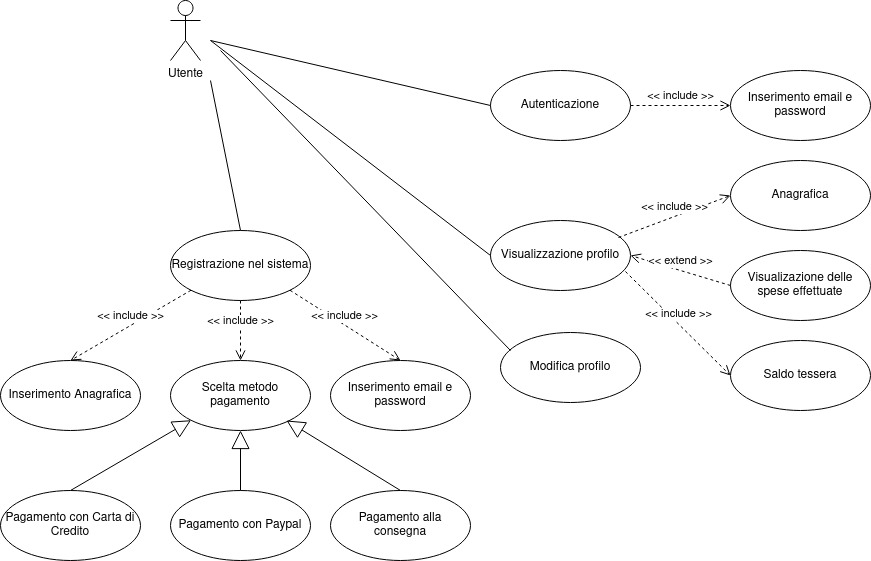
\includegraphics[width=\textwidth]{UseCaseUtenteGestioneProfilo.jpg}
	\caption{Use case di utente per la gestione del profilo e la registrazione}
	\label{fig:UseCaseUtenteGestioneProfilo}
\end{figure}

\newpage


\paragraph{Registrazione nel sistema:}

\begin{mdframed}

	\noindent\textit{\textbf{Attori :}}


	Utente

	\noindent\textit{\textbf{Descrizione :}}


	Procedura di inserimento dei dati dell’utente per registrarsi nel
	sistema

	\noindent\textit{\textbf{Sequenza di eventi :}}


	L’utente inserisce i suoi dati relativi all'anagrafica,
	scelta di metodo di pagamento preferito, email e password.

	\noindent\textit{\textbf{Post condizioni:}}


	Il sistema registra l’utente con i dati inseriti

	\noindent\textit{\textbf{Sequenza Alternativa :}}


	Se i dati inseriti non sono validi il sistema non effettua la
	registrazione
	Se l'email è già stata inserita nel sistema,
	il sistema ne richiede una diversa
\end{mdframed}

\begin{figure}[h!]
	\centering
	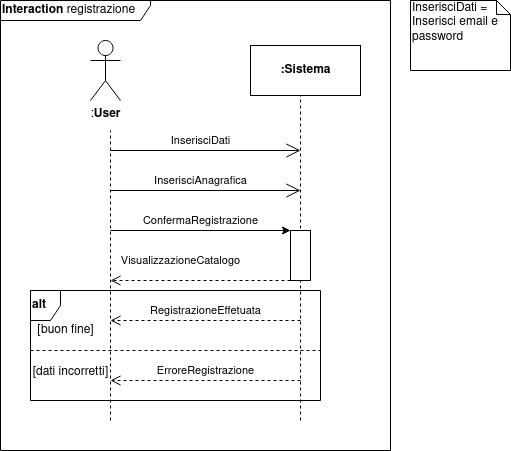
\includegraphics[width=\textwidth]{SDregistrazione.jpg}
	\caption{Sequence Diagram della registrazione}
	\label{fig:SDregistrazione}
\end{figure}
\newpage
\paragraph{Autenticazione:}
\begin{mdframed}

	\noindent\textit{\textbf{Attori :}}


	Utente

	\noindent\textit{\textbf{Descrizione :}}


	Procedura di autenticazione dell'utente

	\noindent\textit{\textbf{Sequenza di eventi :}}


	L’utente inserisce i dati necessari per l'autenticazione

	\noindent\textit{\textbf{Pre-condizioni:}}


	L'utente deve essere registrato nel sistema

	\noindent\textit{\textbf{Sequenza Alternativa :}}


	Se i dati inseriti non sono validi il sistema non effettua
	l'autenticazione

\end{mdframed}

\begin{figure}[h!]
	\centering
	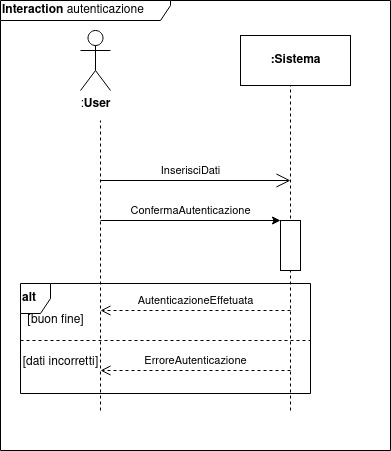
\includegraphics[width=\textwidth]{SDautenticazione.jpg}
	\caption{Sequence Diagram dell'autenticazione}
	\label{fig:SDautenticazione}
\end{figure}

\clearpage
\paragraph{Visualizzazione catalogo:}

\begin{mdframed}
	\noindent\textit{\textbf{Attori :}}


	Utente

	\noindent\textit{\textbf{Descrizione :}}


	Il sistema permette di visualizzare tutti i prodotti disponibili, e ordinarli:
	\begin{enumerate}
		\item in modo crescente e decrescente per prezzo
		\item in ordine alfabetico per marca (dalla A alla Z e dalla Z alla A)
	\end{enumerate}

	\noindent\textit{\textbf{Sequenza di eventi :}}


	L’utente accede all'area dedicata

\end{mdframed}

\paragraph{Gestione profilo:}

\begin{mdframed}
	\noindent\textit{\textbf{Attori:}}


	Utente


	\noindent\textit{\textbf{Scopo e Descrizione sintetica:}}


	Il sistema permette all’utente di gestire il proprio profilo.
	L’utente può visualizzare e modificare il proprio profilo.

	\noindent\textit{\textbf{Sequenza di eventi :}}

	Questo caso d’uso viene attivato quando l’utente vuole modificare o visualizzare il proprio profilo.
	\begin{enumerate}
		\item L’utente sceglie la funzione richiesta
		\item Uno dei seguenti casi d’uso viene utilizzato:
		      \begin{enumerate}
			      \item{ Modifica profilo:
			            comprende la modifica dell'anagrafica.}
			      \item{Visualizzazione profilo: comprende la visualizzazione\\dell'anagrafica,
			            delle spese effettuate e l'attuale saldo punti della tessera.}
		      \end{enumerate}
	\end{enumerate}

	\noindent\textit{\textbf{Pre condizioni:}}


	L’utente deve essere registrato ed aver fatto il login 	nel sistema

	\noindent\textit{\textbf{Post-condizioni:}}


	Se le operazioni di modifica vanno a buon fine lo stato del profilo viene modificato,
	altrimenti il profilo rimane invariato.

	\noindent\textit{\textbf{Sequenza Alternativa:}}


	Se i dati inseriti non sono validi il sistema non effettua modifiche.
\end{mdframed}
\newpage

\subsubsection{Gestione carrello:}

\begin{figure}[h!]
	\centering
	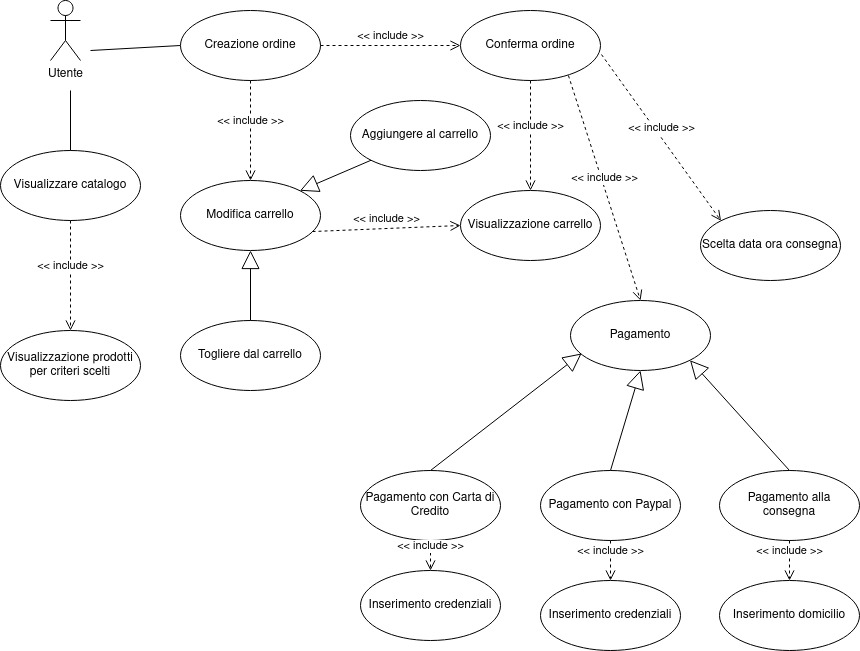
\includegraphics[width=\textwidth]{UseCaseUtenteGestioneCarrello.jpg}
	\caption{Use case del carrello}
	\label{fig:UseCaseUtenteGestioneCarrello}
\end{figure}

\newpage
\begin{mdframed}

	\noindent\textit{\textbf{Attori :}}


	Utente

	\noindent\textit{\textbf{Scopo e Descrizione sintetica :}}


	Il sistema permette all’utente di gestire il proprio carrello della spesa.
	L’utente può visualizzare il proprio carrello,
	inserire prodotti e togliere i prodotti già inseriti e confermare l’ordine.

	\noindent\textit{\textbf{Sequenza di eventi :}}


	\hspace{\parindent} Questo caso d’uso viene attivato quando l’utente vuole modificare il proprio carrello.
	\begin{enumerate}
		\item L’utente sceglie la funzione richiesta
		\item Uno dei seguenti casi d’uso viene utilizzato:
		      \begin{enumerate}
			      \item Modifica al carrello(aggiungere e togliere prodotti)
			      \item Visualizzazione carrello
			      \item Conferma ordine:
			            Viene richiesta la data, l'ora di inizio e  di fine in cui può avvenire la consegna della spesa.
			            Il metodo di pagamento utilizzato per effettuare la spesa è quello scelto dall'utente durante la fase di registrazione o di modifica del profilo.
		      \end{enumerate}
	\end{enumerate}

	\noindent\textit{\textbf{Pre condizioni:}}


	L’utente deve essere registrato ed aver fatto il login 	nel sistema

	\noindent\textit{\textbf{Post-condizioni:}}


	Se le operazioni di modifica vanno a buon fine lo stato del carrello viene modificato,
	altrimenti il contenuto del carrello rimane invariato.
	Se la scelta della data e orario di consegna vanno a buon fine l’acquisto viene fatto, altrimenti l’acquisto
	non viene effettuato.

	\noindent\textit{\textbf{Sequenza Alternativa :}}


	Se durante la conferma il prodotto non è disponibile, viene visualizzato un
	messaggio di errore per informare l’utente che il prodotto non è disponibile.
	Se i dati inseriti non sono validi il sistema non effettua modifiche.
\end{mdframed}
\newpage
\begin{figure}[h!]
	\centering
	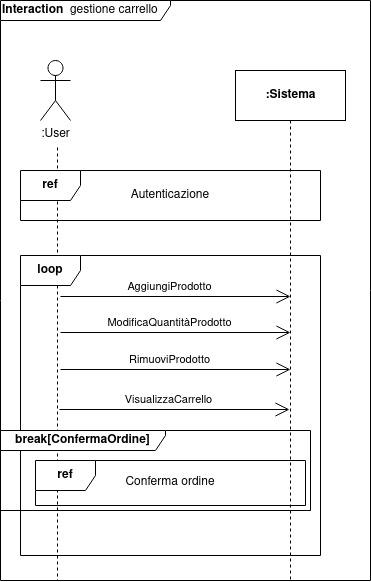
\includegraphics[width=\textwidth]{SDGestioneCarrello.jpg}
	\caption{Sequence Diagramm della gestione del carrello}
	\label{fig:SDGestioneCarrello}
\end{figure}

\begin{figure}[h!]
	\centering
	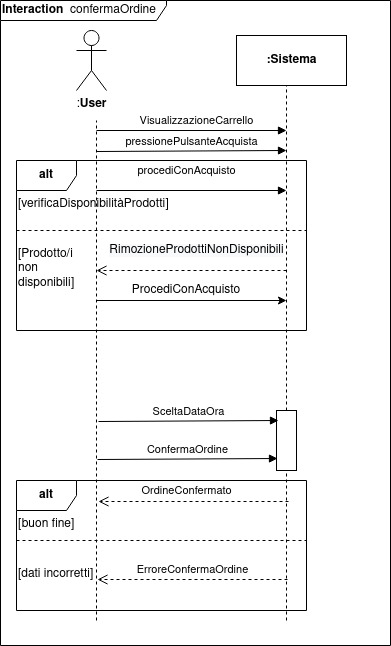
\includegraphics[width=\textwidth]{SDConfermaOrdine.jpg}
	\caption{Sequence Diagramm della conferma dell'ordine}
	\label{fig:SDConfermaOrdine}
\end{figure}
\newpage
\clearpage
\subsubsection{Casi d'uso relativi al responsabile reparto}

\begin{figure}[h!]
	\centering
	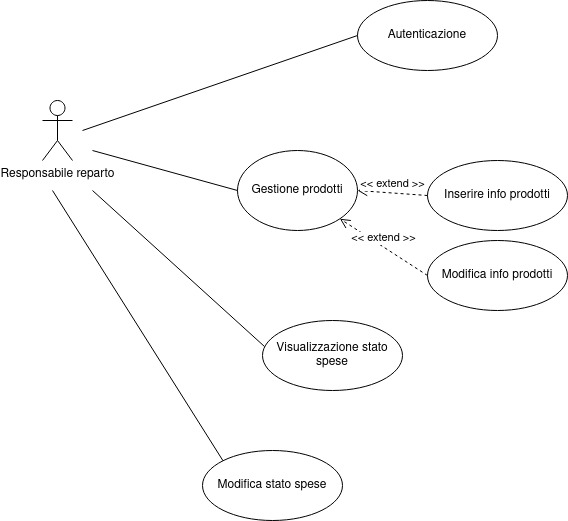
\includegraphics[width=\textwidth]{UseCaseResponsabile.jpg}
	\caption{Use case di responsabile reparto per l'autenticazione la gestione delle spese e dei prodotti}
	\label{fig:UseCaseResponsabile}
\end{figure}

\paragraph{Autenticazione:}
\begin{mdframed}

	\noindent\textit{\textbf{Attori :}}


	Responsabile reparto

	\noindent\textit{\textbf{Descrizione :}}


	Procedura di autenticazione del responsabile di reparto

	\noindent\textit{\textbf{Sequenza di eventi :}}


	Il responsabile inserisce i dati necessari per l'autenticazione

	\noindent\textit{\textbf{Pre-condizioni:}}


	Il responsabile deve essere presente nel sistema

	\noindent\textit{\textbf{Sequenza Alternativa :}}


	Se i dati inseriti non sono validi il sistema non effettua
	l'autenticazione

\end{mdframed}

\paragraph{Visualizzazione stato spese:}
\begin{mdframed}

	\noindent\textit{\textbf{Attori :}}


	Responsabile reparto

	\noindent\textit{\textbf{Descrizione :}}


	Sono visualizzati i dati relativi alle spese dei clienti.

	\noindent\textit{\textbf{Sequenza di eventi :}}


	Il responsabile accede all'area dedicata

	\noindent\textit{\textbf{Pre-condizioni:}}


	Il responsabile di reparto aver fatto il login nel sistema


	\noindent\textit{\textbf{Sequenza alternativa:}}


	Se i dati inseriti non sono validi il sistema non effettua modifiche

\end{mdframed}

\paragraph{Gestione prodotti}

\begin{mdframed}

	\noindent\textit{\textbf{Attori :}}


	Responsabile reparto

	\noindent\textit{\textbf{Descrizione :}}


	Il sistema permette al responsabile di gestire i prodotti del proprio reparto
	Con la possibilità di modificare e aggiungere i prodotti che sono terminati o che stanno
	per terminare.
	Inotre può inserire nel sistema nuovi prodotti che appariranno sul catalogo

	\noindent\textit{\textbf{Sequenza di eventi :}}


	Il responsabile accede all'area dedicata

	\noindent\textit{\textbf{Pre-condizioni:}}


	Il responsabile di reparto aver fatto il login nel sistema

	\noindent\textit{\textbf{Sequenza alternativa:}}


	Se i dati inseriti non sono validi il sistema non effettua modifiche
\end{mdframed}

\newpage
\section{Sviluppo: progetto dell'architettura ed implementazione del sistema}
\subsection{Note sul processo di sviluppo}
\subsection{Progettazione e pattern architetturali usati}
\subsubsection{Pattern MVC}
Il progetto è strutturato con il Pattern MVC, perché fornisce una coerenza strutturale solida
semplificando le fasi di progettazione e implementazione. Inoltre crea un'ottima sinergia con la
piattaforma JavaFX.

\noindent Il sistema è suddiviso in tre parti:
\begin{itemize}
	\item{\textbf{Model:}
	      Sono presenti le classi che definiscono i dati manipolati
	      e implementano la logica businnes.
	      Inoltre sono presenti le classi che permettono la comunicazione
	      con il Database organizzate seguendo il DAO pattern.
	      }
	\item{\textbf{View:}
	      Parte esclusivamente dedicata alla visualizzazione dei dati
	      presenti nel modello.
	      In particolare si utilizzano file del formato fxml per rappresentare
	      l'interfaccia grafica.
	      }
	\item{\textbf{Controller:}
	      Le classi Controller sono utilizzate come mezzo di comunicazione
	      tra il Model e la View, permettono l'interazione dell'utente con il
	      sistema e implementano della logica per validare i dati inseriti dall'utente.
	      }
\end{itemize}

\subsection{Pattern Repository}
\noindent La memorizzazione dei dati avviene attraverso l'utilizzo di un database centrale chiamato Spesa nella quale è stata creata una tabella per ciascuna classe che implementa il DAO pattern.

Le motivazioni che hanno portato alla scelta del repository pattern sono la semplicità d'uso e la centralità del sistema di recupero delle informazioni infatti è necessaria una sola classe per creare la connessione con il database ed eseguire le query (vedi classe ConnectionDb).
\subsection{Note su JavaFX}
L'implementazione dell'interfaccia grafica è stata fatta utilizzano file fxml costruiti con SceneBuilder.
Questo permette di comporre in modularmente l'interfaccia grafica.
In varie parti del progetto si utilizza una vista che viene richiamata più volte per generare un contenuto
dinamico all'interno di una vista più complessa.(Es. Vedi Catalogo, contiene più istanze di un Prodotto)
\subsection{Implementazione e design pattern usati}
\subsubsection{Pattern Sigleton}
Il pattern singleton è stato utilizzato nell'implementazione della classe ConnectionDb, allo scopo di
instaurare una connessione con il database, eseguire interrogazioni generiche e recuperare i risultati.
L'oggetto connectionDb viene istanziato una volta all'avvio dell'applicativo e viene utilizzato
da tutta le classi DaoImpl contenti le interrogazioni effettive.
\begin{figure}[h!]
	\centering
	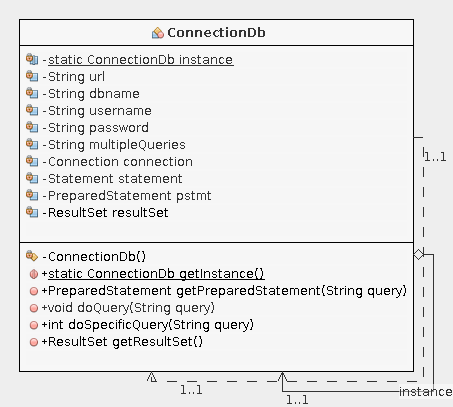
\includegraphics[width=\textwidth]{UmlConnectionDb.png}
	\caption{UML della classe ConnectionDb}
	\label{fig:UmlProdotto}
\end{figure}
\newpage

\subsubsection{Pattern Observer e gestione della sessione} 
Durante lo sviluppo si è presentata la necessita di terner traccia dello stato di alcune istanze di oggetti che
sono e visualizzati o modificati in più viste.
Per asempio se aggiungiamo al carrello un prodotto nel catalogo ci aspettiamo che la lista di prodotti nel
carrello sia aggiornata inserendo il prodotto scelto.
Per risolvere il problema di un'istanza di un oggetto condivisa tra più viste utilizziamo la classe SessionStorage
alla quale si è applicato il pattern Subject-Observer per notificare il cambiamento di stato.


\noindent Quindi la classe \textbf{SessionStorage} svolge il ruolo di \textbf{Subject} che notifica agli 
Observer il cambiamento del suo stato.


\noindent Le classi \textbf{Controller} hanno il ruolo di \textbf{Observer} ad aggiornano la vista quando
il Subject cambia stato.

\begin{figure}[h!]
	\centering
	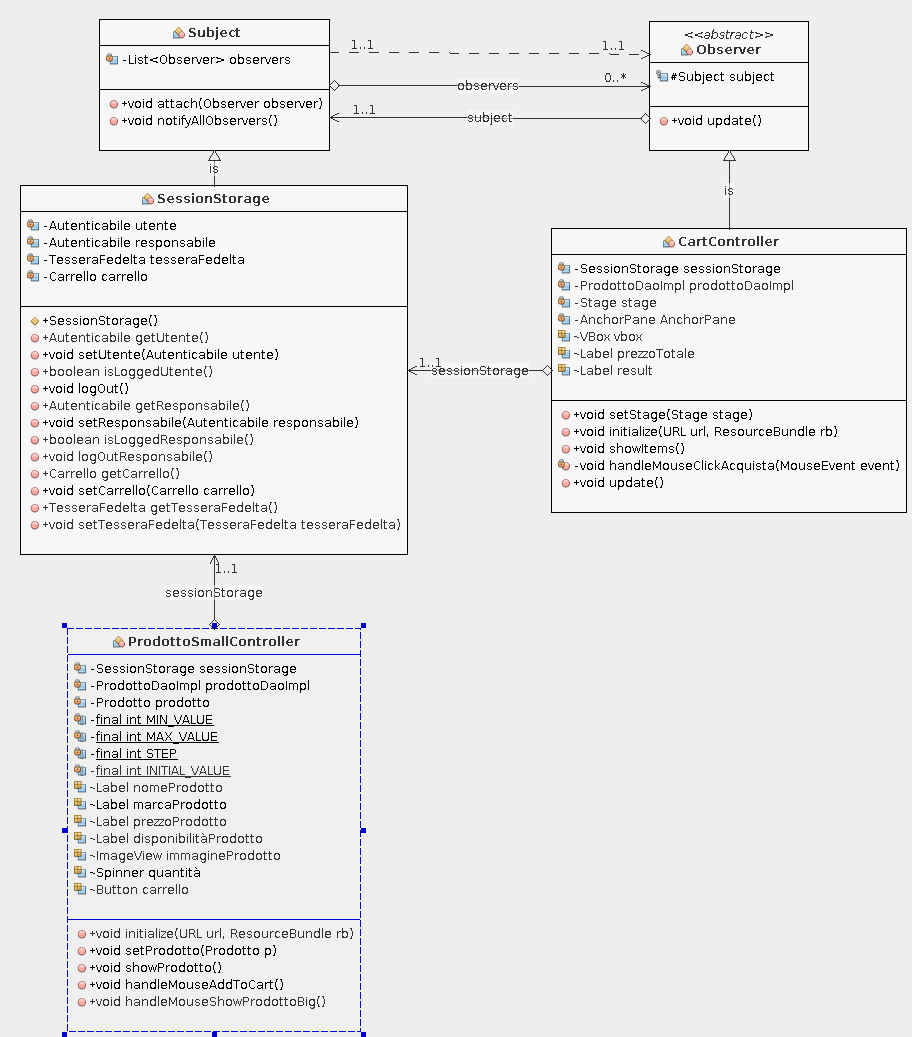
\includegraphics[width=\textwidth]{UmlObserver.png}
	\caption{UML delle classi che utiliazzano il pattern Observer}
	\label{fig:UmlProdotto}
\end{figure}
\newpage
\subsubsection{Pattern Data Access Object}
\begin{figure}[h!]
	\centering
	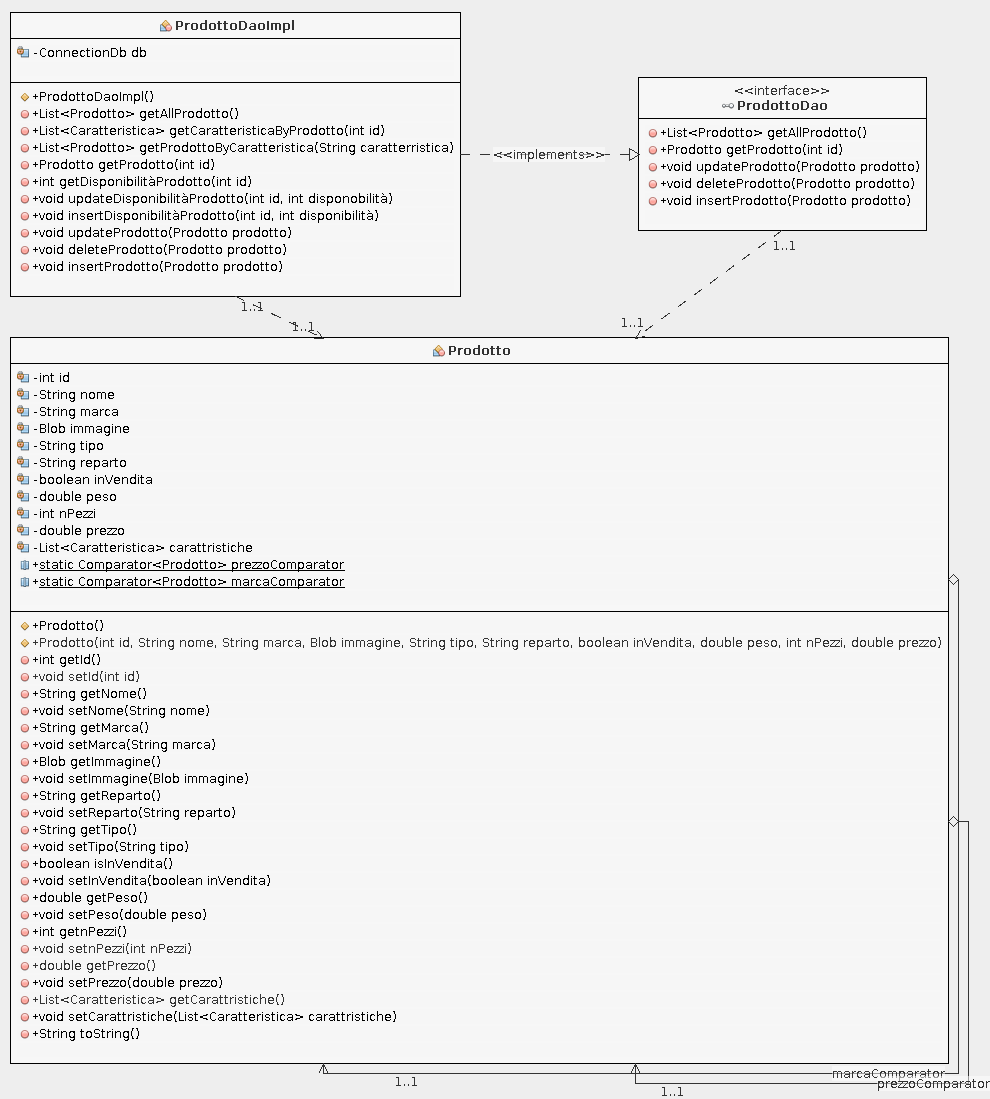
\includegraphics[width=\textwidth]{UmlProdotto.png}
	\caption{UML della classe Prodotto con pattern DAO}
	\label{fig:UmlProdotto}
\end{figure}

\subsubsection{UML delle Classi}
\begin{figure}[h!]
	\centering
	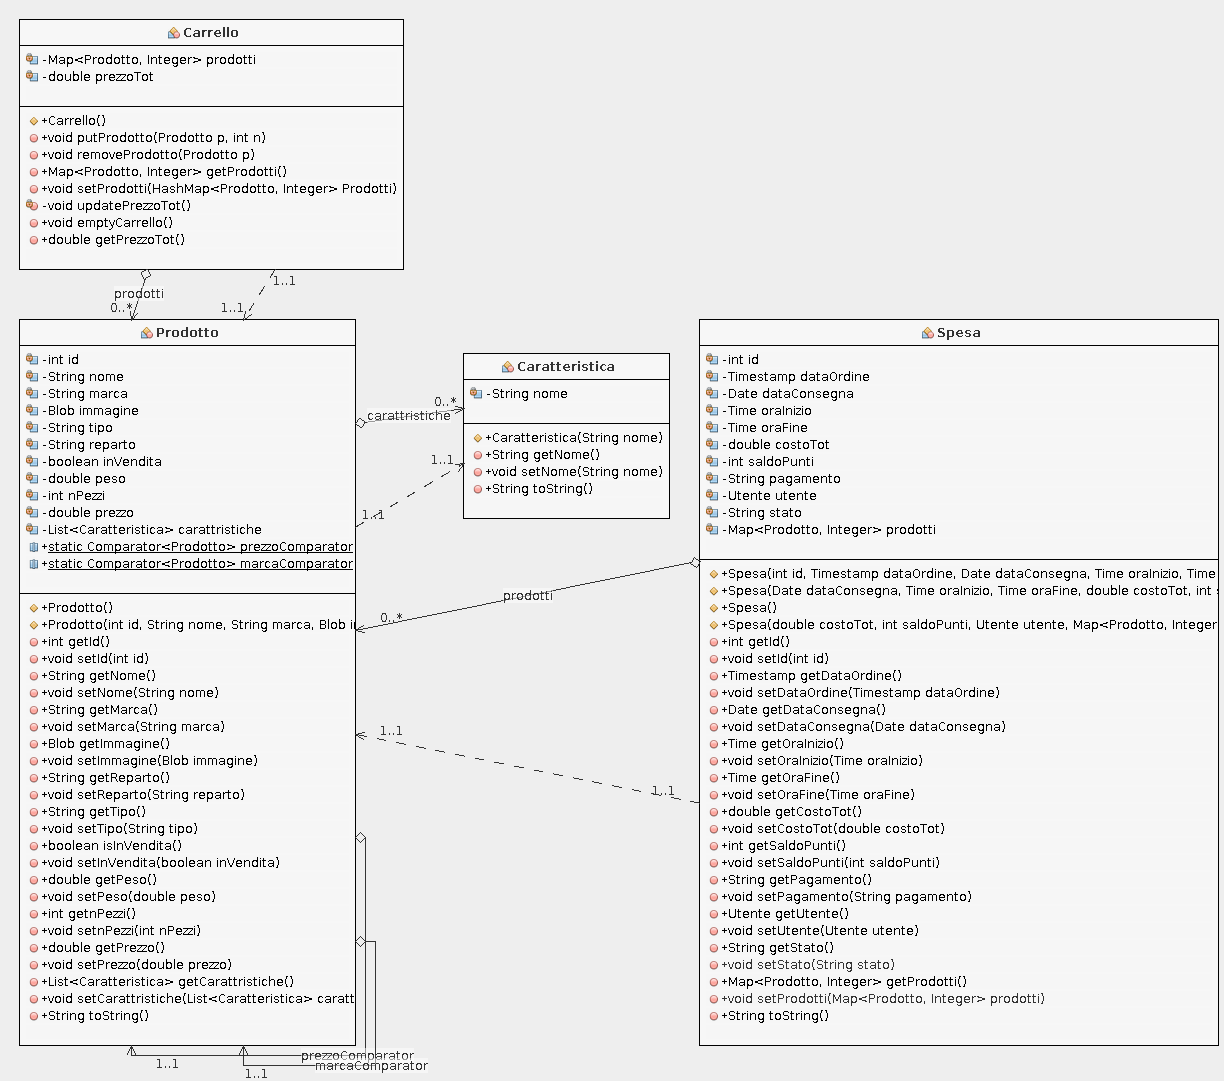
\includegraphics[width=\textwidth]{UmlSpesa.png}
	\caption{UML della classe Spesa e Carrello in relazione con Prodotto presenti nel model} 
	\label{fig:UmlSpesa}
\end{figure}


\begin{figure}[h!]
	\centering
	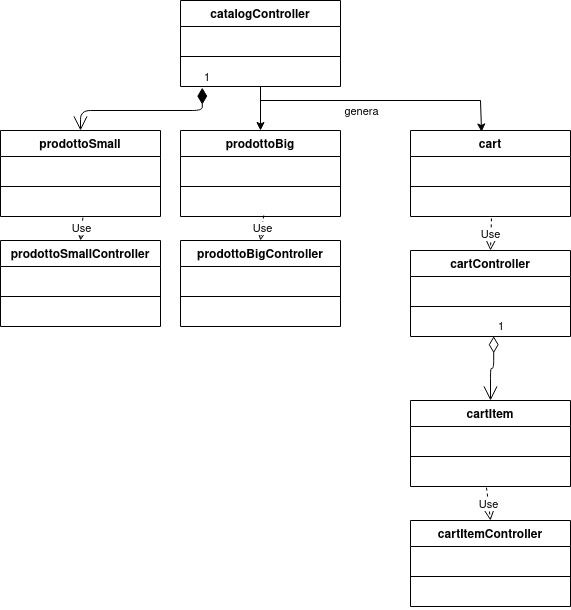
\includegraphics[width=\textwidth]{UmlCatalog.jpg}
	\caption{UML delle classi della vista Catalogo}
	\label{fig:UmlCatalog}
\end{figure}

\begin{figure}[h!]
	\centering
	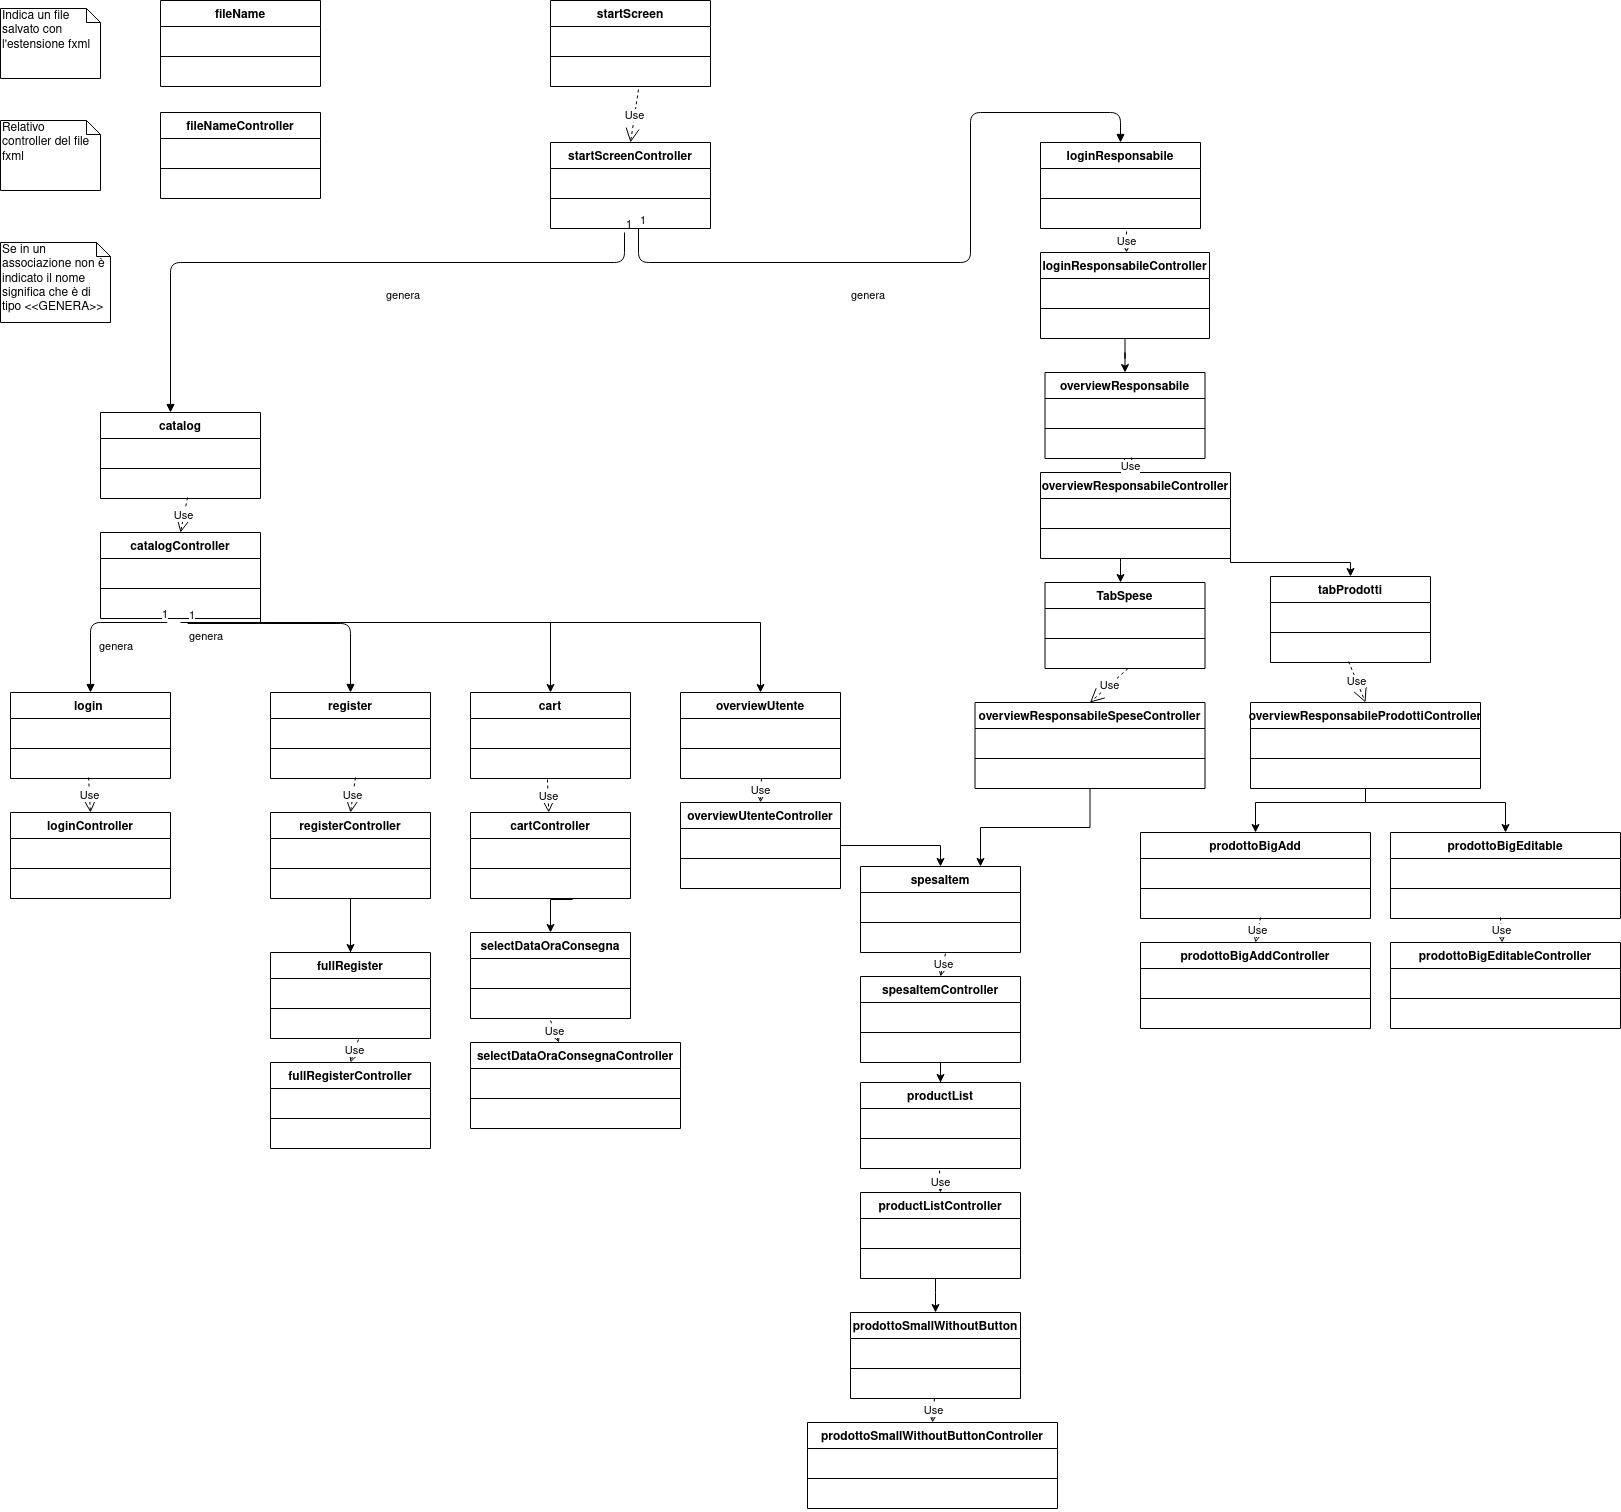
\includegraphics[width=\textwidth]{UmlInterfaccie.jpg}
	\caption{UML delle Classi di tutte le viste}
	\label{fig:UmlInterfaccie}
\end{figure}

\clearpage
\subsection{Persistenza dati con Database SQL}
Utilizzare un database ha portato i seguenti vantaggi:
\begin{itemize}
	\item{
	      L'applicativo può utilizzare un qualsiasi database remoto specificando l'indirizzo e le credenziali d'accesso.}

	\item{
	      Possibilità di utilizza più istanze contemporaneamente dell'applicativo affidando la gestione
	      della concorrenza al DBMS.}
	\item{
	      Accesso e modifica dei dati facilitato con l'utilizzo delle interrogazioni.}
\end{itemize}

\subsubsection{Diagramma ER}

\begin{figure}[h!]
	\centering
	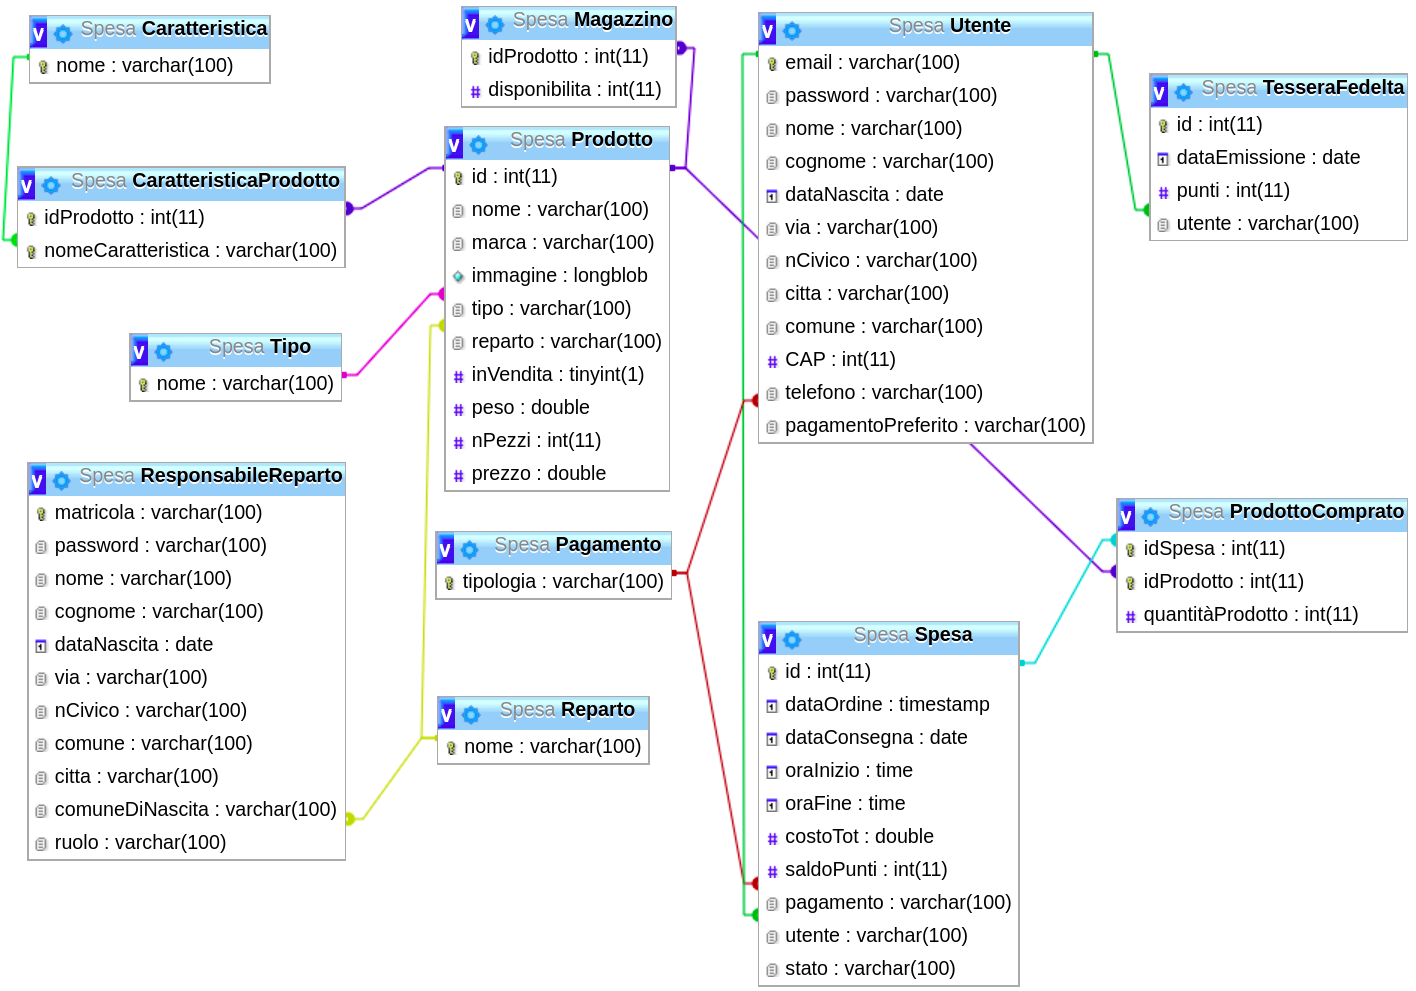
\includegraphics[width=\textwidth]{DiagrammaER.png}
	\caption{Diagramma Entity Relationship}
	\label{fig:DiagrammaER}
\end{figure}

\end{document}
